% Instructions to change to html version:
% Comment out:
%  minipage, multicols,columnbreak, mathbf, hrule
% Replace all: \begin{minipage}% \end{minipage} %\begin{mulicols}  %\end{mulicols}  %\columnbreak % \begin{framed} %\end{framed} %\hrule
% Search for \mathbf
% Replace $$ with \[ and $ with \(
% Enclose graphics in figure environments and add captions
% Re-tag \df environments as sections, subsections, etc.
% Command Line Code to Create html version:
%First: pdflatex -shell-escape filename.tex                                   
%Second, for each figure: inkscape "filename-figure1.pdf" -o "filename-figure1.png"
% Third: htlatex filename.tex "ht5mjlatex.cfg, charset=utf-8" " -cunihtf -utf8"
\documentclass[10pt]{article}

%\usepackage{tikz, pgf,pgfplots,wasysym,array}
%\usepackage{wasysym,array}

\usepackage{amsmath,amssymb}

\ifdefined\HCode
  \def\pgfsysdriver{pgfsys-tex4ht-updated.def}
\fi 
%\ifdefined\HCode
%  \def\pgfsysdriver{pgfsys-dvisvgm4ht.def}
%\fi 
\usepackage{tikz}
\usetikzlibrary{calc,decorations.markings,arrows}
\usepackage{pgfplots}

\pgfplotsset{compat=1.12}
\usepackage{myexternalize}
\usetikzlibrary{calc,decorations.markings,arrows}
\usepackage{framed}
\usepackage[none]{hyphenat}

\input{../../../common/1336_header_test.tex}
% \input{header.tex}

\usepackage{multirow, array}
\begin{document}

\everymath{\displaystyle}

\renewcommand{\myTitle}{MATH 1336: Calculus III}

\renewcommand{\mySubTitle}{Section 1.2: Calculus with Parametric Curves, Part 1}
%~\hfill Name: \underline{~~~~~~~~~~~~~~~~~~~~~~~~~~~~~~~~~~~~~~~~~~~~~~~}

\lectTitle{\vspace*{-.5in}\myTitle}{\vspace*{.1in}\mySubTitle \vspace*{-.25in}}


\setlength{\columnseprule}{0.4pt}
\setlength{\columnsep}{3em}

%\hspace*{-.8in}\begin{minipage}{1.25\textwidth}
%\begin{framed}

\section*{Differential Calculus with Parametric Curves:}

%\begin{minipage}{.4\textwidth}

\begin{figure}[!h]
\includegraphics[width=\textwidth]{parametric-tangent.png}
\caption{Figure showing a line tangent to a parametric curve at a point P.}
\end{figure}

% \end{minipage}
%\hspace*{.1in}
%\begin{minipage}{.6\textwidth}
Consider a point \(P\) on a parametric curve \(C\) that has coordinates given by
\[
P: (x(t), y(t)).
\]

We would like to extend the concepts of \textbf{slope} and \textbf{concavity} from Differential Calculus to the new setting of parametric curves.\\~\\
%\underline{\textbf{\Large Potentially Useful Formulas:}}\\~\\
%\small
\textbf{Slope:}
\[
\frac{dy}{dx} = \dfrac{\frac{dy}{dt}}{\frac{dx}{dt}} = \dfrac{y'(t)}{x'(t)}\]

Note that the tangent line will be: \textbf{horizontal} at points where \(y'(t) = 0\),\\ 
\textbf{vertical} at points where  \(x'(t) = 0\).\\

To find an equation for the tangent line, you can use the  the point-slope equation of a line:
\[y - y_1 = m(x-x_1)\]

\textbf{Concavity:}
\[
\frac{d^2y}{dx^2} = \dfrac{\frac{d}{dt}\left(\frac{dy}{dx}\right)}{x'(t)}\]
%
%\vspace*{-.2in}
% \end{minipage}
%\end{framed}
% \end{minipage}

\section*{Example:}
\begin{enumerate}[{Example} 1:]
\addtocounter{enumi}{1}

\item Consider the parametric curve 
\[
x = 3 - 2t - t^2, \quad y = t^3+3t^2-2, \quad -3 \leq t \leq 1.
\]
We will use the following steps to draw a rough sketch of the curve without using a calculator or Mathematica.\\~\\


%\begin{minipage}{.25\textwidth}
\hspace*{-.75in}
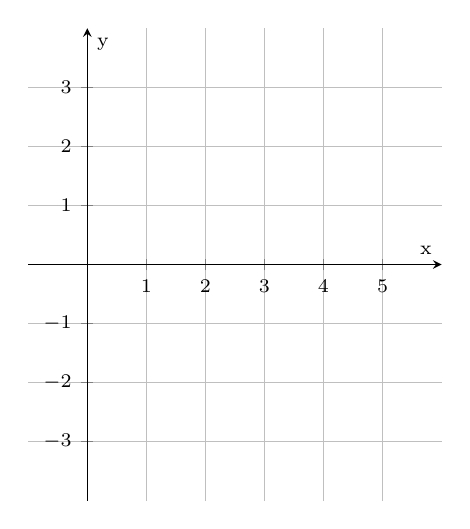
\begin{tikzpicture}
\begin{axis}[
	x=.75cm,
    y=.75cm,
	axis x line=middle,
	axis y line = middle,
	xmin=-1,xmax=6,
	ymin=-4,ymax=4,
    grid=both,
%    ticks=none,
%    yticklabels={},
%    xticklabels={},
    xtick={0,1,...,5},
    ytick={-3,-2,...,3},
    xlabel=x,
    ylabel=y,
    label style={font=\scriptsize},
    tick label style={font=\scriptsize}
]



\end{axis}
%\filldraw[fill=green!20,draw=green!50!black] (1.5cm,0cm) -- (3.75cm,0cm) arc
%(0:45:3.75cm) -- (1.065cm,1.065cm) arc (45:0:1.5cm) -- cycle;
%
%

\end{tikzpicture}
% \end{minipage}
\hspace*{-.25in}
%\begin{minipage}{.7\textwidth}
\begin{enumerate}[(a)]
\item Determine the locations of any points on the curve where the tangent line is either horizontal or vertical. \label{horiz-vert}
\vspace*{.2in}
\item Plot and label the points found in part \ref{horiz-vert}, as well as the initial and terminal point.\label{points}
\vspace*{.2in}
\item In order to connect the points from part \ref{points} in the correct order, note that the curve must intersect itself. How can we find the locations of the intersection point(s)?
\vspace*{.2in}
\end{enumerate}

% \end{minipage}
\end{enumerate}
%\vfill
\begin{flushright}
\textit{(Mathematica Demo: Parametric Calculus)}
\end{flushright}
\pagebreak

\section*{Problems for Group Work:}


\begin{enumerate}[{Problem} 1:]
\addtocounter{enumi}{-1}

\item Introduce yourself to your partners and tell everyone about a new skill or hobby that you have learned/enjoyed recently.

\vfill



\item As \(t\) varies, the following parametric equations trace out a line in the \(xy-\)plane
\[
x = 2 + 3t, \qquad y= 4+7t
\]
\begin{enumerate}
%\item What part of the line is obtained by restricting \(t\) to nonnegative numbers?
%\item What part of the line is obtained if \(t\) is restricted to \(-1\leq t\leq 0\)?
%\item How should \(t\) be restricted to give the part of the line to the left of the \(y-\)axis?
\item Calculate \(\frac{dy}{dx}\) to determine the slope of the line.
\item Eliminate the parameter to find a Cartesian equation of the line.\\ Use this equation to check your work from the previous part of the problem.
\item Calculate \(\frac{d^2y}{dx^2}\). Does your result match with your intuition regarding the concavity of a line?
\end{enumerate}

\vfill


\item Consider the curve parametrized by
\[
x=3\cos(t), \qquad y=2\sin(t), \qquad 0\leq t \leq 2\pi.
\]
\begin{enumerate}
\item Sketch a graph of the curve, and indicate the direction  in which the curve is traced as \(t\) increases.\\
\textit{Hint:} What would the graph look like if the coefficients on the trig functions were the same?
%\item Find \(\frac{dy}{dx}\) and \(\frac{d^2y}{dx^2}.\)
\item Find an equation for the line tangent to the curve at the point where \(t=\pi/6\). 
\item Does your tangent line equation make sense, given the graph of the curve?
\item Use calculus to find the points on the curve where the tangent line is horizontal or vertical. Compare your solutions with the graph to check your work.
%\item Use the graph to determine for which values of \(t\) the curve is concave up.
\item Find \(\frac{d^2y}{dx^2}\). Determine for which values of \(t\) the curve is concave up.\\ Use the graph to check your work.
\item Eliminate the parameter to find a Cartesian equation of the curve.
\end{enumerate}
\vfill


\end{enumerate}

\end{document}
